
%%%%%%%%% MASTER -- compiles the 4 sections

\documentclass[11pt,letterpaper]{article}

\usepackage{graphicx}
\usepackage{verbatim}
\usepackage{listings}
\usepackage{amssymb,amsmath}
\usepackage{enumerate}

%%%%%%%%%%%%%%%%%%%%%%%%%%%%%%%%%%%%%%%%%%%%%%%%%%%%%%%%%%%%%%%%%%%%%%%%%
\pagestyle{plain}                                                      %%
%%%%%%%%%% EXACT 1in MARGINS %%%%%%%                                   %%
\setlength{\textwidth}{6.5in}     %%                                   %%
\setlength{\oddsidemargin}{0in}   %% (It is recommended that you       %%
\setlength{\evensidemargin}{0in}  %%  not change these parameters,     %%
\setlength{\textheight}{8.5in}    %%  at the risk of having your       %%
\setlength{\topmargin}{0in}       %%  proposal dismissed on the basis  %%
\setlength{\headheight}{0in}      %%  of incorrect formatting!!!)      %%
\setlength{\headsep}{0in}         %%                                   %%
\setlength{\footskip}{.5in}       %%                                   %%
%%%%%%%%%%%%%%%%%%%%%%%%%%%%%%%%%%%%                                   %%
\newcommand{\required}[1]{\section*{\hfil #1\hfil}}                    %%
\renewcommand{\refname}{\hfil References Cited\hfil}                   %%
\bibliographystyle{plain}                                              %%
%%%%%%%%%%%%%%%%%%%%%%%%%%%%%%%%%%%%%%%%%%%%%%%%%%%%%%%%%%%%%%%%%%%%%%%%%

%PUT YOUR MACROS HERE

\date{Due April May 11th, 2012}
\title{CS 452 Final Exam}

\author{Colby Blair}

\begin{document}
\maketitle

\begin{center}

Grade: \_\_\_\_\_\_\_\_\_\_\_\_\_\_\_\_\_\_\_\_
\end{center}

\thispagestyle{empty}

\pagebreak


\section*{1}

\subsection*{a)}
The C language was not designed for the Harvard architecture, with its seperate program (flash) and 
data (RAM) memory. It is challenging to get some things like constant data in program space, so it can
be used efficiently, using C. Asking for more data (malloc) and accessing address space requires the 
compiler to do a lot more work, and if the compiler doesn't make the efficient decisions, then the 
programmer may want to step in (i.e. using the PROGMEM macro).

\subsection*{b}
If I wrote a language for embedded systems, I would write a language that was strictly data and resource 
driven. It seems like we had to write a lot of code in C to figure out what our resources were, where they 
were located in memory space, and where the data lived as well. A language that allowed the programmer 
to simply tie resources and data to whatever memory space would take a lot of work out of things. The 
language could then come with libraries or features to do things like resource management, mutex, 
semphores, and scheduling easily. It would just require the programmer to identify the addresses where
stuff lived.

\section*{2}
Any functionality that could be kept in standards C could be included in the general purpose O/S. The 
O/S would have to leave things like interrupts, timers, i/o, special locking operations, and anything else 
hard dependent up to the developer to add / create. To me, these would be like kernel modules. The O/S
should be able to assume that a call to an interrupt, timer, or hardware resource locking does the same thing
conceptually, regardless of the actual implemenation. 

Although this may not be exactly true, the O/S 
kernel modules for particular hardware could make the hardware perform to the O/S assumptions. Some
efficiency may be lost due to the lack of using the hardware to its full potential, but the result would be an
O/S that could run on many types of hardware. This is probably a trade off of any software written for
multiple kinds of hardware.


\section*{3}
\subsection*{Binary semaphores}
Binary semaphores, like mutex semaphores, have only two states; taken or not taken. The difference is that
binary semaphores cannot be owned. Therefore, they are useful for public resources in the system that 
need service by tasks. This could be things like hardware or events in an event queue.

\subsection*{Mutex semaphores}
Mutex semaphores, like binary semaphores, have two states, but mutex's can be owned. They are useful 
when a task needs to lock a resource (like a port) that involve operations in its critical section. This can 
potentially lead to a situation of priority inversion, where a task owns a resource but is suspended, and the
higher priority task is mutexed out of using it. The optimization for this is to write a schedule that can
detect these priority inversions / deadlocks.

\subsection*{Counting semaphores}
Counting semaphores are typically used to guard resources that are available in discrete quantities. One
example of this are used slots in a circular queue.


\section*{4}
In virtual memory, each task can own pages that map to collections of physical memory somewhere,
either loaded more locally (registers or RAM), or more isolated (discs on the system). This can simplify
memory management and protection from the tasks's perspective, but adds a lot of overhead in the
embedded system world. 

Like the RTOS I reported on, simpler memory management is used, where the 
physical hardware memory maps closer to the address space that tasks see, than virtual memory.
This cuts down on overhead, but doesn't allow for things like memory fragmentation. Since embedded
system memory is generally pretty low, these lacks of features generally aren't a problem.


\section*{5}
Priority inversions happen when a task that is of a lower priority holds a resource (i.e. via a mutex 
semaphore), is suspended by a task of higher priority, and that task is then waiting on that resource to
be freed. The higher priority task must essentially hand runtime back over to the lower priority task, or it
will hang the system waiting for the locked resource. This nullifies its higher priority. 

Solutions include disabling interrupts when a priority inversion prone resource is consumed, but is not 
favorable, because it can run away with the OS, and disables preemption. Another approach is priority
inheritance, which means that when a lower priority tasks create a priority inversion, that lower priority task
is temporarily assigned a higher priority so it can finish. Another approach is to create
priority thresholding, which allows only tasks with certain priorities to interrupt other tasks. This means
that tasks that could priority invert each other should stay in the same group. 


\section*{6}
\begin{tabular}{ | c | c | c | }
	\hline
	step	&	hardware								&	software \\
	\hline
	1	&	program counter (PC) is pushed to stack		& \\
	\hline
	2	&	address from interrupt vector table jumped to & \\
	\hline
	3	&										& push general purpose (GP) registers to stack \\
	\hline
	4	&										& push status register (SR) to stack \\
	\hline
	5	&										& store the current stack pointer (SP) \\
	\hline
	6	&										& set SP to new task \\
	\hline
	7	&										& restore new task SR \\
	\hline
	8	&										& restore new task GP \\
	\hline
	9	&	PC is restored from stack					& \\
	\hline
\end{tabular}


\section*{7}
\subsection*{a)}
The problem with the textbf{bypass capacitor} is that it probably doesn't really buffer the circuit from the
spike that the switch might put off. It does decouple the power requirements a bit from the switch by providing a little extra current during dips in power, but probably only takes out small, brief powe spikes.

\subsection*{b)}
The symptoms would be still a noticable spike coming from the switch, and if the switch spikes things 
when the capacitor is fully charged (switched off and on quickly), the power spike might be worse than
without the capacitor.

\subsection*{c)}
One solution would be to create an RC circuit to ease incoming amperage / power. The resistor in the RC
circuit reduces the amperage coming in, and increases the charge time of the capacitor. At first, the 
voltage over the capacitor to ground is 0V and over the resistor is the source voltage. As the capacitor
charges from the incoming current, the voltage increases across it until it matches source. At this point,
the voltage over the resistor is 0V.

\begin{figure}[!h]
        \begin{center}
		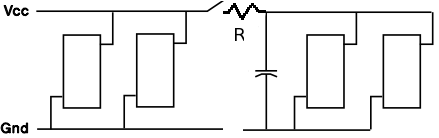
\includegraphics[width=120mm]{images/rc_circuit}
                \caption{RC circuit solution}
                \label{tool_layout}
        \end{center}
\end{figure}

The voltage curve measure at the positive side of the capacitory can be determined from the RC time
constant. The effect of the gradual voltage increase here is a solution to buffering power spikes from the
switch.


\section*{8}
\subsection*{bitset}
\lstinputlisting{src/bitset.h}

\subsection*{bitclr}
\lstinputlisting{src/bitclr.h}

\subsection*{allset}
\lstinputlisting{src/allset.h}

\subsection*{allclr}
\lstinputlisting{src/allclr.h}

\subsection*{setval}
\lstinputlisting{src/setval.h}

\subsection*{setabs}
\lstinputlisting{src/setabs.h}


\section*{9}
\subsection*{a)}
The equations for Rate Monotonic response time is given as:
\begin{eqnarray}
	R_i = C_i + \sum_{j \epsilon hgp(i)}^{} (\frac{R_i}{T_j})C_j
	w_{i}^{n + 1}
\end{eqnarray}

For processes:

\begin{tabular}{ c c c c }
	process	&	T (period)		& C (computation time) 	& Priority \\
	1		&	6			& 1.5 				& 1 \\
	2		&	5			& 2 					& 2 \\
	3		&	4			& 1 					& 3 \\
\end{tabular}

We calculate response time as follows:
\begin{eqnarray}
	R_1 = \frac{3}{2} \\
	w_{2}^{0} = 2 \\
	w_{2}^{1} = 2 + \lceil \frac{2}{6} \rceil \frac{3}{2} = \frac{7}{2} \\
	w_{2}^{2} = 2 + \lceil \frac{\frac{7}{2}}{6} \rceil \frac{3}{2} = \frac{7}{2} \\  	
	R_2 = \frac{7}{2} \\
	\\
	w_{3}^{0} = 1 \\
	w_{3}^{1} = 1+ \lceil \frac{1}{6} \rceil \frac{3}{2} + \lceil \frac{1}{5} \rceil 2 
			= \frac{9}{2} \\
	w_{3}^{2} = 1+ \lceil \frac{\frac{9}{2}}{6} \rceil \frac{3}{2} + \lceil \frac{\frac{9}{2}}{5} \rceil 2 
			= \frac{9}{2} \\
	w_{3}^{3} = 1+ \lceil \frac{\frac{9}{2}}{6} \rceil \frac{3}{2} + \lceil \frac{\frac{9}{2}}{5} \rceil 2 
			= \frac{9}{2} \\
	w_{3}^{4} = 1+ \lceil \frac{\frac{9}{2}}{6} \rceil \frac{3}{2} + \lceil \frac{\frac{9}{2}}{5} \rceil 2 
			= \frac{9}{2} \\
	w_{3}^{5} = 1+ \lceil \frac{\frac{9}{2}}{6} \rceil \frac{3}{2} + \lceil \frac{\frac{9}{2}}{5} \rceil 2 
			= \frac{9}{2} \\
	\\
	R_3 = \frac{9}{2}
\end{eqnarray}

So we can rewrite the table as follows:

\begin{tabular}{ c c c c  c }
	process	&	T (period)		& C (computation time) 	& Response	& Utilization \\
	1		&	6			& 1.5 				& 1.5 		& .25 \\
	2		&	5			& 2 					& 3.5 		& .50 \\
	3		&	4			& 1 					& 4.5 		& .25 \\
\end{tabular}

This gives us a \textbf{combined utilization} of 1.0. This is above the threshold of \textbf{.78} for three
processes, but the process set \textbf{will meet its deadlines}. This means that the task set 
\textbf{does have a feasible static priority assignment}.

\subsection*{b)}
A calculated above, the \textbf{load / combined utilization} is 1.0.

\pagebreak

\subsection*{c)}
Considering the table again:

\begin{tabular}{ c c c c  c }
	process	&	T (period)		& C (computation time) 	& Response	& Utilization \\
	1		&	6			& 1.5 				& 1.5 		& .25 \\
	2		&	5			& 2 					& 3.5 		& .50 \\
	3		&	4			& 1 					& 4.5 		& .25 \\
\end{tabular}

These lead to the following Earliest Deadline First schedule:

\begin{figure}[!h]
        \begin{center}
		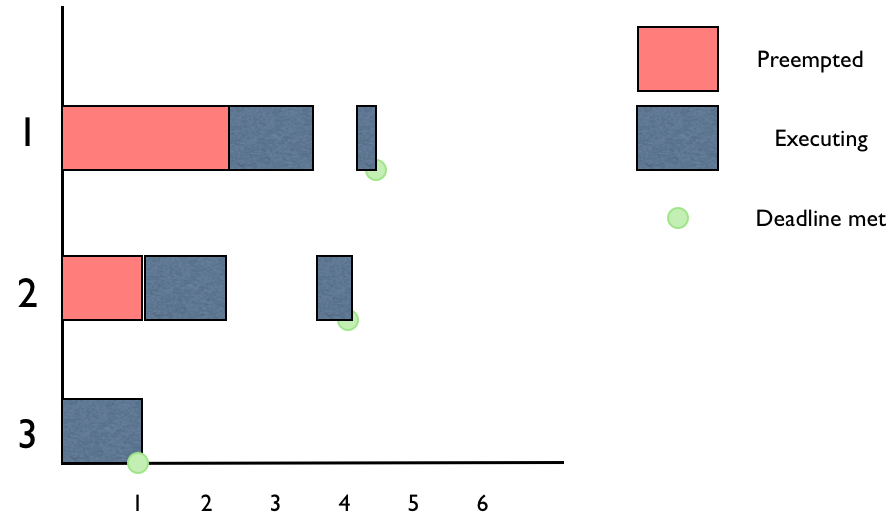
\includegraphics[width=120mm]{images/deadline_first}
                \caption{Earliest Deadline First schedule}
                \label{deadline_first}
        \end{center}
\end{figure}

\end{document}